\documentclass{article}
\usepackage{algpseudocode,algorithm,algorithmicx}
\usepackage[usenames,dvipsnames,svgnames,table]{xcolor}
\usepackage[hidelinks]{hyperref} 
\usepackage{graphicx}
\usepackage{amsmath} 

\begin{document}
    \title{\textcolor{blue}{\textbf{Informe Proyecto de EDA II \\Temario 7}}\\}
    
    % \author{\\David Orlando De Quesada Oliva C211\\Daniel de la Cruz Prieto C211\\ Javier Dominguez C212} 
    \date{} 
    \maketitle  

    \begin{abstract}
        \noindent En este informe  vamos a resolver los 4 problemas del proyecto final de 
        EDA~2. Para cada problema vamos a dar  una explicaci\'on breve de como se resuelve el mismo, demostrar todo el marco te\'orico necesario, 
        pseudoc\'odigo, correctitud y complejidad temporal del algoritmo.\\\\
        \\\\
        \\\\
        \\\\
        % El trabajo esta en un repositorio de GitHub en el siguiente enlace 
        % \href{ https://github.com/dcruzp/Proyecto-de-EDA}{\textcolor{blue}{click aqui}}.\\\\
        {\large{ \textcolor{blue}{\textbf{Integrantes :}}}}
        \begin{itemize}
            \item \textbf{David Orlando De Quesada Oliva}  C-211
            \item \textbf{Daniel de la Cruz Prieto} C-211
            \item \textbf{Javier E. Dominguez Hern\'andez} C-212
        \end{itemize}
        % La Bibliografia fundamental fue las conferencias de Clases , Ademas de algunos libros de Teorias de Grafos como son : 
        % \begin{itemize}
        %     \item Introducti\'on to Algorithm 3er Edition
        %     \item Graph Algoritm 2nd Edition , Shimon Even 
        % \end{itemize}
       
    \end{abstract}

    \newpage 

    \setcounter{tocdepth}{2}
    \tableofcontents

    \newpage 


    \section{Problema 1}
    
    \subsection{\underline{Orden del problema}} 

    Sean n casas en un vecindario y m tuber\'ias. Las tuber\'ias de agua subterr\'aneas conectan estas casas. Cada
    tuberı\'ia tiene cierta direcci\'on (el agua puede fluir solo en esta direcci\'on y no al rev\'es) y di\'ametro (que caracteriza
    la cantidad m\'axima de agua que puede manejar).
    \\[10pt]
    \noindent Para cada casa, hay como m\'aximo una tuber\'ia entrando y como m\'aximo una tuber\'ia saliendo de ella. Se quiere
    instalar tanques y grifos en las casas. Para cada casa con una tuber\'ia de agua saliente y sin una tuber\'ia de agua
    entrante, se debe instalar un tanque de agua en esa casa. Por cada casa con una tuber\'ia de agua entrante y
    sin una tuber\'ia de agua saliente, se debe instalar un grifo de agua en esa casa. Cada casa tanque transportar\'a
    agua a todas las casas que tengan una secuencia de tuber\'ias desde el tanque hasta ella. En consecuencia, cada
    casa de grifo recibir\'a agua procedente de alguna casa de tanque.
    \\[10pt]
    \noindent Para evitar que las tuber\'ias exploten una semana después tambi\'en se debe considerar el di\'ametro de las tuber\'ias.
    La cantidad de agua que transporta cada tanque no debe exceder el di\'ametro de las tuber\'ias que conectan un
    tanque a su correspondiente grifo. Se quiere encontrar la cantidad m\'axima de agua que se puede transportar de
    forma segura desde cada tanque hasta su grifo correspondiente. Dise\~ne un algoritmo que devuelva la cantidad
    m\'axima de agua que se puede trasnportar de forma segura desde cada tanque hasta su grifo correspondiente.
    La complejidad temporal de su algoritmo debe ser de \textit{O(n + m)}.
    
    \subsection{\underline{Soluci\'on}}

    Primero que todo consideremos el conjunto de casas del vecindario como los v\'ertices, y las tuber\'ias como las aristas de un grafo
    dirigido  $G$, las aristas tienen una funci\'on de capacidad (di\'ametro de la tuber\'ia) y los v\'ertices tienen a lo sumo $indegree = 1$
    y a lo sumo $outdegree$ = 1 por las restricciones del problema.\\\\

    \noindent \textbf{Definici\'on:} Una casa con tanque $u$ en el grafo $G$ es un $u \in V(G)$,\\ $indegree(u) = 0 \wedge outdegree(u) = 1$\\

    \noindent \textbf{Definici\'on:} Una casa con grifo $u$ en el grafo $G$ es un $u \in V(G)$,\\ $indegree(u) = 1 \wedge outdegree(v) = 0$\\

    \noindent \textbf{Definici\'on:} Diremos que a la casa con tanque $u$, en el grafo $G$, le corresponde la casa con grifo
     $v$, si existe un camino de $u$ a $v$ en $G$.\\

     \noindent \textbf{Definici\'on:} Diremos que a la casa con grifo $v$ en el 
    grafo $G$, le corresponde la casa con tanque $u$, si existe un camino de $u$ a $v$ en $G$.\\\\

    \noindent \textbf{Proposici\'on 1:} A cada casa con tanque $u \in V(G)$ le corresponde una \'unica casa con grifo $v \in V(G)$.\\

    Supongamos que a una casa con tanque $u \in V(G)$ le corresponde al menos dos casas con grifo, eso quiere decir
    que hay un camino de $u$ a cada una de dichas casas. Tomemos dos de dichas casas y los caminos $p_1, p_2$ de $u$
    a cada una de ellas, pueden ocurrir dos cosas con dichos caminos:\\\\

    $\bullet$ Los caminos $p_1$ y $p_2$ solo tienen en com\'un el v\'ertice $u$ (casa con tanque). En este caso
    el $outdegree(u) \geq 2$ (al menos tiene grado dos, pues solo tomamos estos dos caminos, pero pueden haber m\'as que
    solo tengan a $u$ como v\'ertice com\'un).\\

    $\bullet$ Los caminos $p_1$ y $p_2$ tienen en com\'un m\'as de un v\'ertice. En este caso comencemos recorriendo $p_1$ desde
    $u$, y sea $w$ el \'ultimo v\'ertice com\'un con $p_2$ en $p_1$, se cumple que $outdegree(w) \geq 2$ (pueden que hayan mas caminos
    que lleguen a $w$ por el mismo recorrido que $p_1, p_2$).\\\\

    En ambos casos llegamos a una contradicci\'on con las restricciones del problema, que es que $\forall x \in V(G), outdegree(x) \leq 1$. 
    Por tanto a cada casa con tanque $u$ le corresponde una \'unica casa con grifo $v$.\\\\

    \noindent \textbf{Proposici\'on 2:} A cada casa con grifo $u \in V(G)$ le corresponde una \'unica casa con tanque $v \in V(G)$.\\

    Supongamos que a la casa con grifo $u$ le corresponden al menos dos casas con tanque, eso quiere decir que hay al menos dos casas
    con tanque tal que hay un camino de cada una de ellas a la casa con grifo $u$. Tomemos dos de dichas casas y los caminos $p_1, p_2$,
     que van de cada una de ellas a la casa con grifo $u$, pueden ocurrir dos cosas con dichos caminos:\\\\

    $\bullet$ Los caminos $p_1$ y $p_2$ solo tienen en com\'un el v\'ertice $u$ (casa con grifo). En este caso
    el $indegree(u) \geq 2$ (al menos tiene grado dos, pues solo tomamos estos dos caminos, pero pueden haber m\'as que
    solo tengan a $u$ como v\'ertice com\'un)\\
 
    $\bullet$ Los caminos $p_1$ y $p_2$ tienen en com\'un m\'as de un v\'ertice. En este caso comencemos recorriendo $p_1$ y $p_2$ desde cada
    uno de sus v\'ertices iniciales hasta $u$, y tomemos el primer v\'ertice com\'un a ambos en dicho recorrido, ese v\'ertice que digamos es $w$
    cumple que $indegree(w) \geq 2$ (pueden que hayan mas caminos que lleguen a $w$)\\\\

    En ambos casos llegamos a una contradicci\'on con las restricciones del problema, que es que $\forall x \in V(G), indegree(x) \leq 1$. 
    Por tanto a cada casa con grifo $u$ le corresponde una \'unica casa con tanque $v$.\\\\

    Por las Proposiciones 1 y 2 se deduce que cada casa con grifo recibe agua de una sola casa con tanque, y una casa con tanque env\'ia agua a
    una sola casa con grifo. Que esto es que los pares $u,v \in V(G)$ tal que $u$ es el tanque que env\'ia agua al grifo $v$, no tienen elementos repetidos.\\\\\

    \noindent \textbf{Proposici\'on 3:} Entre cada casa tanque $u \in V(G)$ y su grifo correspondiente, $v \in V(G)$ hay un \'unico camino
    que va de $u$ a $v$ en $G$ y es un camino simple.\\

    Supongamos que hay al menos dos caminos que van de $u$ a $v$ en $G$. Tomemos dos de dichos caminos, $p_1$ y $p_2$, ambos caminos pueden cumplir solo las 
    siguientes condiciones:\\\\

    $\bullet$ Ambos empiezan en $u$ y el v\'ertice siguiente en ambos caminos es distinto, en este caso $outdegree(u) \geq 2$\\\\
    $\bullet$ Ambos tienen una serie de v\'ertices en com\'un y se separan en alg\'un punto del recorrido antes de llegar a $v$, 
    en este caso tomemos el \'ultimo v\'ertice com\'un a $p_1$ y $p_2$, denotemos ese v\'ertice como $w$, se cumple que $outdegree(w) \geq 2$\\\\

    En ambos casos llegamos a una contradicci\'on con las restricciones del problema, que es que $\forall x \in V(G), outdegree(x) \leq 1$. 
    Por tanto para toda casa con tanque $u$ que env\'ia agua a su correspondiente casa con grifo $v$, se cumple que existe un \'unico camino de $u$ a $v$.\\\\

    Ahora supongamos que ese camino que denotaremos como $p_i$ no es simple, eso quiere decir que hay un ciclo en dicho camino, empecemos a recorrer $p_i$ hasta 
    que lleguemos al primer v\'ertice $x$ que est\'a en dicho ciclo, la arista que usamos para llegar a \'el no estaba en el ciclo y aporta 1 de $indegree$ a $x$,
    y la otra arista, que cierra el ciclo en $x$ aporta 1 de $indegree$, por lo que $indegree(x) = 2$, lo que es una contradicci\'on con las restricciones del problema.\\\\

    Por tanto, el \'unico camino entre $u$ y $v$ en $G$, es simple.\\\\

    Debido a que las proposiciones previamente analizadas son ciertas, el vecindario(casas y tuber\'ias) representado utilizando un grafo dirigido $G$, quedar\'ia de la siguiente forma:\\\\

    \begin{figure}[h]
        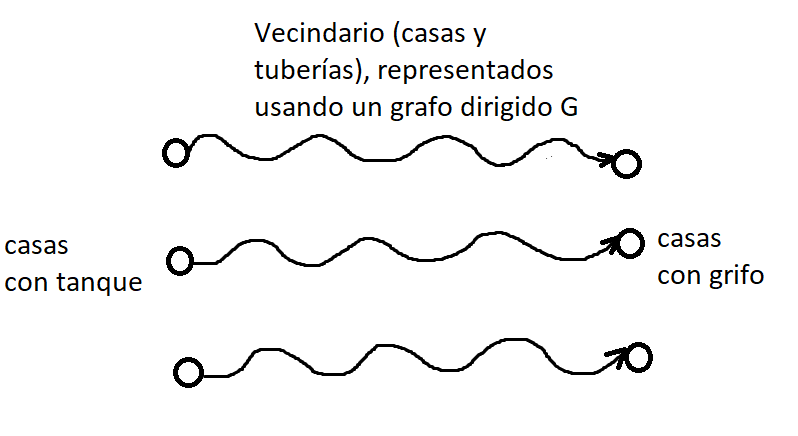
\includegraphics[scale = 0.5]{img/Image1Problem1.png}
        \centering
    \end{figure}

    O sea, el vecindario representado utilizando un grafo dirigido $G$, queda formando varias componentes conexas en el grafo $G$,
    donde cada una de dichas componentes conexas representa un \'unico camino simple que va de una casa con tanque, a su correspondiente
    casa con grifo.\\\\

    Nuestro problema, nos pide hallar la mayor cantidad de agua que se puede transportar desde cada tanque hacia su correspondiente grifo de forma segura, o sea 
    de forma que la cantidad de agua que transporta dicho tanque hacia su grifo, no exceda el di\'ametro de las tuber\'ias que conectan un tanque con su correspondiente
    grifo, que esto es, en el grafo $G$ que representa nuestro vecindario, determinar para cada v\'ertice $w \in V(G)$, $indegree(w) = 0$ y $outdegree(w) = 1$, cual es la cantidad m\'axima
    de flujo que se puede enviar hacia su correspondiente $z \in V(G), outdegree(z) = 0$ y $indegree(z) = 1$, por supuesto, sobre este grafo es imposible  aplicar el concepto de flujo,
    pues no hay una fuente ni un destino, y es para eso que construiremos un nuevo grafo $G'$ de la siguiente forma: agregaremos un v\'ertice ficticio $x$, unido por un arco, a cada uno de los $u \in V(G), indegree(u) = 0$ y $outdegree(u) = 1$, y para cada 
    $<x,u> \in E(G'), c(<x,v>) = \infty$, y haremos un procedimiento parecido para los v\'ertices $v \in V(G), indegree(v) = 1$ y $outdegree(v) = 0$, que es conectarlos por un arco, a un v\'ertice ficticio $y$, y
    para cada $<v,y> \in E(G'), c(<v,y>) = \infty$. De esta forma obtenemos un grafo $G'$, como se muetra a continuaci\'on, donde si es posible aplicar el concepto de flujo estudiado en conferencias, pues dicho grafo es una red de flujo
    dadas las restricciones del problema y las modificaciones explicadas previamente.\\
    
    \begin{figure}[h]
        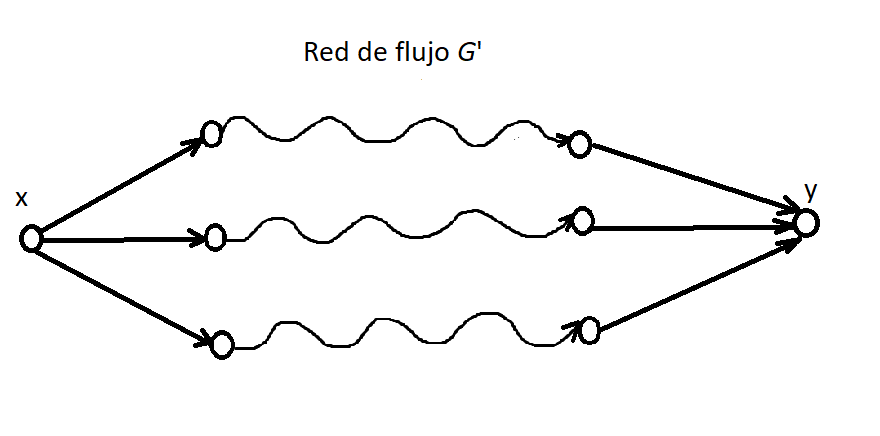
\includegraphics[scale = 0.5]{img/Image2Problem1.png}
        \centering
    \end{figure}

    Dadas las caracter\'isticas del problema en cuesti\'on (hay un \'unico camino entre cada tanque y su grifo correspondiente) y por las proposiciones demostradas previamente, 
    es posible determinar el valor m\'aximo flujo que se puede enviar desde cada tanque a su grifo correspondiente, 
    simplemente haciendo un DFS desde el v\'ertice ficticio $x$, tendremos una lista que denotaremos max, de tama\~no $n$, donde en la posici\'on i, almacenaremos el valor 
    m\'aximo de flujo que se puede enviar desde el tanque i hasta su grifo correspondiente y una variable $min$ que utilizaremos para calcular el flujo m\'aximo para cada 
    tanque, de la siguiente manera. Comenzamos haciendo DFS($G'$,$x$) y por la propia estructura de $G'$ necesariamente, el algoritmo ejecutar\'a DFS-Visit($G'$,$u$), 
    $\forall u \in V(G'), <x,u> \in E(G')$, ya que no hay forma de alcanzar uno de los tanques desde otro y por tanto el DFS-Visit no los marcar\'a como visitados. Ahora simplemente
    en cada camino que vaya desde un tanque a un grifo, vamos almacenando en $min$, la menor de las capacidades en el camino(como las aristas ficticias que a\~nadimos tienen 
    capacidad infinita, no afectar\'a al m\'inimo que estamos computando), una vez regresemos al v\'ertice $x$ por backtrack en el propio DFS, almacenamos en la lista max en la posici\'on 
    que identifica al v\'ertice $u$, el valor de $min$, y reiniciamos el valor de $min$ a $\infty$ para computar el m\'inimo en el siguiente camino entre un tanque y un grifo. No es necesario
    tener en cuenta los v\'ertices $u \in V(G), indegree(u) = 0$ y $outdegree(u) = 0$ pues dichos v\'ertices(en caso de que existan) no aportan nada al c\'omputo que estamos realizando, pues no son 
    alcanzables desde ning\'un otro v\'ertice, ni alcanzan a ning\'un otro v\'ertice en $G$.\\\\ 

    \subsection{\underline{Pseudoc\'odigo}}
    \begin{algorithm}[H]
        \caption{Calcular la capacidad m\'axima de agua que se puede transportar de forma segura desde cada tanque hasta su grifo correspondiente}
        \textbf{Solve($G$)\\}
        1-\hspace*{1em}$G'$ = Build\textunderscore Flow\textunderscore Network($G$) - Este m\'etodo en $O(V)$ agrega los v\'ertices fictios a $G$ .\\
        2-\hspace*{1em}$max \leftarrow$ [$\infty]$*$|V(G')|$ - lista donde tendremos para cada v\'ertice que sea tanque la cantidad m\'axima de flujo que puede enviar a su grifo.\\
        3-\hspace*{1em}$min \leftarrow \infty$ - esta variable la usaremos para computar lo que nos pide el ejercicio\\
        4-\hspace*{1em}visited $\leftarrow$ [$false$]*$|V(G')|$, $\pi \leftarrow$ [$Null$]*$|V(G')|$\\
    
        5-\hspace*{1em}\textbf{DFS($G'$, $x$)}\\
        6-\hspace*{2em}$min \leftarrow \infty$\\
        7-\hspace*{2em}\textbf{for each} $u \in Ady[x]$ do:\\
        8-\hspace*{3em}DFS-Visit($G'$, $u$)\\
        9-\hspace*{3em}$max$[$u$] $\leftarrow min$\\
        10-\hspace*{3em}$min \leftarrow \infty$\\

        11-\hspace*{1em}\textbf{DFS-Visit$(G,u)$}\\ 
        12-\hspace*{2em}u $\leftarrow$ visited \\  
        13-\hspace*{2em}\textbf{for each} v $\in$ $Adj[u]$\\
        14-\hspace*{3em}do \textbf{if} v not visited\\
        15-\hspace*{4em}$\pi[v] \leftarrow u$\\
        16-\hspace*{4em}do \textbf{if} $c(u,v)< min$\\
        17-\hspace*{5em}$min=c(u,v)$\\
        18-\hspace*{4em}DFS-Visit($G$,$v$)\\
        
        19-\hspace*{1em}\textbf{for each} $u \in V(G')$\\
        20-\hspace*{2em}\textbf{if} $max$[$u$] != $\infty$\\
        21-\hspace*{3em}\textbf{print}($u$,$max$[$u$]) - la capacidad m\'axima de agua que puede transportar el tanque u a su correspondiente grifo es $max[u]$\\
        
    \end{algorithm}

    \subsection{\underline{Correctitud}}

    La correctitud de nuestro algoritmo, se debe a la correctitud del DFS demostrada en conferencia, y al cumplimiento de las proposiciones 
    1, 2 y 3 previamente demostradas, y que son una consecuencia de las restricciones impuestas en la orden del problema. Lo que
    agregamos al DFS para actualizar min y max no afecta para nada la corretitud del mismo.\\

    \subsection{\underline{Complejidad Temporal}}
    La complejidad de nuestro algoritmo se basa en la complejidad del DFS $O(n + m)$. Lo \'unico que le agregamos al DFS
    es ir actualizando  el m\'inimo de las capacidad de las aristas que participan en un camino desde un tanque hasta un 
    grifo lo cual no afecta la complejidad temporal del mismo. Construir la red de flujo $G'$ es $O(n)$ y hacer un recorrido por el array max
    para imprimir las casas que son tanque, con la m\'axima capacidad correspondiente que se puede transportar de forma segura 
    desde el mismo hasta su grifo, tiene complejidad $O(n)$. La complejidad temporal de nuestro algoritmo, por tanto, quedar\'ia $O(n) + O(n + m) + O(n) 
    = O(max(n + m, n)) = O(n + m)$.



    \newpage 

    \section{Problema 2} 

    \subsection{\underline{Orden del Problema}}
    
    Dise\~ne un algoritmo que dado un grafo no dirigido con costo en las aristas $G = <V, E>$ y los v\'ertices x, $y \in  V$ ,
    determine el costo de la arista de menor costo entre las aristas de mayor costo en cada camino de x a y. Esto
    quiere decir que si de x a y existen dos caminos $P_1$ , $P_2$ y la arista de mayor costo en $P_1$ es 5 y la de mayor costo
    en $P_2$ es 4, entonces deben devolver 4. La complejidad temporal de su algoritmo debe ser de $O(|E|log(|V|))$.\\

    \subsection{\underline{Soluci\'on}}

    \noindent \textbf{Proposici\'on 1 :} \\
    
    Sea $G = <V,E>$ grafo no dirigido con costo en las aristas, $x$, $y$ $\in V(G)$, $y$ alcanzable desde $x$, \textbraceleft$p_1, p_2,..., p_t$\textbraceright 
    los caminos de $x$ a $y$ en $G$, \textbraceleft$e_1, e_2,..., e_t$\textbraceright las aristas de costo m\'aximo en cada uno de los caminos $p_i$, $1 \leq i \leq t$, y
    $E'$ = \textbraceleft $e \in E(G) |\hspace{0.2em} w(e)$ = min \textbraceleft $w(e_i) |\hspace{0.2em} 1 \leq i \leq t$ \textbraceright \textbraceright, el conjunto
    de las aristas de menor costo entre las $e_i$. Entonces el algoritmo de PRIM tomando como v\'ertice inicial $x$, devuelve un AACM $T$ de $G$, tal que $\exists\hspace{0.2em}
    e' \in E', e' \in E(T)$ y el \'unico camino de $x$ a $y$ en el AACM $T$ pasa por $e'$.\\\\
    
    Inicialmente, como est\'a descrito en conferencia en la cola con prioridad que mantiene el corte(o sea el conjunto de v\'ertices a\'un no visitados por el algoritmo)est\'an todos los 
    v\'ertices del grafo G. En cada paso del algoritmo se a\~nade una nueva arista de forma tal que siempre se mantiene un conjunto de aristas que son un subcojunto de alg\'un AACM $T$ de $G$,
    como se describe en la conferencia. Por esto, en alg\'un momento del algoritmo $\exists\hspace{0.2em} e'' = \hspace{0.2em}<u,v>\hspace{0.2em} \in E'$ que ser\'a la arista candidata a 
    a\~nadir al conjunto de aristas que se tiene hasta el momento, y puede ocurrir dos cosas :\\\\
    
    $\bullet$ Que se a\~nada dicha arista, o sea, que el v\'ertice $v$ a\'un no haya sido alcanzado por el algoritmo usando alg\'un otro camino de $x$ a $y$. En este caso ya tenemos que cuando 
    se termine de ejecutar el algoritmo se cumplir\'a que $\exists e' \in E', e' \in E(T)$ donde $T$ es el AACM resultante al terminar el algoritmo de PRIM.\\\\

    $\bullet$ Que no se a\~nada dicha arista, o sea, que el v\'ertice $v$ haya sido alcanzado por el algoritmo, usando otro de los caminos que van de $x$ a $y$.
    Digamos q ese camino fue $p_k$, entonces $e_k$ no puede tener costo mayor que $e''$, pues, en dicho caso, el propio algoritmo garantiza que se tome la arista de menor costo
    de todas las que cruzan el corte y en dicho caso ser\'ia $e''$, por lo tanto $v$ no puede haber sido alcanzado usando $p_k$, lo que es una contradicci\'on pues asumimos que $v$
    fue alcanzado usando $p_k$. Por tanto la \'unica posiblidad es que $e_k \in E'$, o sea $e_k$ es una de las aristas que tiene costo m\'inimo entre todas las aristas
    de mayor costo en cada camino de $x$ a $y$ ($w(e_k) = w(e''))$, y por tanto se cumple que $e_k \in E', e_k \in E(T)$ donde $T$ es el AACM resultante al terminar el algoritmo de PRIM.\\\\

    $\Rightarrow$ Por tanto al finalizar el algoritmo de PRIM, ejecutado sobre  el grafo $G$, iniciando en el v\'ertice $x$, se cumple que 
    $\exists e' \in E', e' \in E(T)$, siendo $T$ el AACM resultante al terminar el algoritmo de PRIM.\\\\

    Sea $e' = <u,v>$, hay un \'unico camino de $x$ a $u$ en $T$, y hay un \'unico camino de $v$ a $y$ en $T$, y como consecuencia de que esta arista est\'a en todo AACM $T$ de $G$
    $\Rightarrow$ hay un \'unico camino de $x$ a $y$ en $T$ que pasa por la arista $e'$\\\\

    $\bullet$ Por tanto se cumple la proposici\'on 1\\\\
    %\newpage
    \subsection{\underline{Pseudoc\'odigo}}
    \begin{algorithm}[H]
        \caption{Determinar el costo de la arista de menor costo entre las aristas de mayor costo en cada camino de $x$ a $y$ en un grafo $G$ con funci\'on de costo $w$}
        \textbf{Solve($G,x,y,w$)\\} 
        1-\hspace*{1em}$T$ $\leftarrow$ PRIM($G,x,w$) --------- Construir un AACM de $G$ empezando en $x$. $O(|E|\log{|V|})$\\
        2-\hspace*{1em} \textbf{if} $\pi$[y] != NULL:\\
        3-\hspace*{2em}start $\leftarrow y$, answer $\leftarrow$ $w(\pi[y],y)$. $O(1)$\\ 
        4-\hspace*{2em}\textbf{while} start != $x$ do:  $O(|E|)$\\
        5-\hspace*{3em}start $\leftarrow$ $\pi$[start] $O(1)$\\
        6-\hspace*{3em}answer $\leftarrow$ m\'ax(answer,w($\pi$[start],start)) $O(1)$\\
        7-\hspace*{2em} return answer\\\\
        
        l\'ineas 3-7 Quedarse con el mayor de los costos de las aristas en el camino de $x$ a $y$ en $T$
    \end{algorithm}

    \subsection{\underline{Correctitud}}

    La correctitud del algoritmo se basa principalmente en la del algoritmo de PRIM visto en conferencia, y en esencia en 
    la aplicaci\'on de la proposici\'on 1 previamente demostrada, una vez verificado que $y$ es alcanzable desde $x$, utilizando el array 
    $\pi$, que computa el propio algoritmo de PRIM al construir el AACM empezando en $x$, solo resta quedarse con la arista de mayor costo 
    en el camino de $x$ a $y$ en $T$, operaci\'on que realizan las l\'ineas 3-7 del pseudoc\'odigo usando el array $\pi$.

    \subsection{\underline{Complejidad Temporal}}
    La complejidad temporal del algoritmo se base en la complejidad de PRIM que es $O(|E|\log{|V|})$. El recorrido 
    que se hace por el array $\pi$, para quedarse con la arista de mayor costo en el camino de $x$ a $y$ en $T$, tiene complejidad $ O(|E|)$. 
    Entonces la complejidad temporal del algoritmo es:\\ $O(|E|\log{|V|}) + O(|E|) = O(max(|E|\log{|V|}, |E|)) = O(|E|\log{|V|})$

    \newpage 


    \section{Problema 3} 

    \subsection{\underline{Orden del problema}} 

    Sea $G = <V,E>$ un grafo no dirigido y conexo con pesos positivos en las aristas, y un v\'ertice $s \in V$ . Un \'arbol de 
    caminos de costo m\'inimos con ra\'iz en s es un subgrafo $T = <V^{'} , E^{'}> $ donde $V^{'} \subseteq  V $     y $E^{'} \subseteq  E $ tal que: 
    
    \begin{itemize}
        \item $V^{'}$ es el conjunto de v\'ertices alcanzables desde s en $G$
        \item $T$ es un \'arbol con ra\'iz en $s$
        \item Para todo $v \in V^{'}$ el \'unico camino simple de $s$ a $v$ en $T$ es un camino de costo m\'inimo de $s$ a $v$ en $G$ .
    \end{itemize}

    \noindent Dise\~ne un algoritmo que encuentre en el grafo G un \'arbol T de caminos de costo m\'inimo con ra\'iz en s tal que
    la suma de los pesos de las aristas de T sea lo menor posible. La complejidad temporal del algoritmo debe ser
    $O(|E|log|V|)$.


    \subsection{\underline{Soluci\'on }}

    \noindent La soluci\'on al problema es aplicar el algoritmo de  Dijkstra visto en conferencias.
    Para encontrar un subgrafo $G^{'}$ que contenga todas las aristas que forman parte de alg\'un camino de 
    costo minimo desde $s$ hasta cualquier otro v\'ertice del grafo $G$. Luego encontramos un \'arbol $T$ abarcador de 
    costo m\'inimo en $G^{'}$ , $T$ es el \'arbol que estamos buscando 


    
    \subsubsection{Proposiciones }
    \begin{itemize}
        \item Vamos a denotar $\delta\left(u,v\right)$ como la distancia m\'inima de $u$ a $v$ 
        \item Vamos a denotar a $w(u,v)$ como el peso de la arista $e= <u,v>$ 
        \item Sea $G = <V,E>$ un grafo, vamos a denotar a $G' = <V',E'>$ como un subgrafo de $G$ que solo contiene las aristas $ u \xrightarrow[]{e} v$, 
        que cumplen que $\delta\left(s,u\right) + w \left(u,v\right) = \delta\left(s,v\right)$   
    \end{itemize}

    \subsubsection{Lema 1:}

    \textit{Sean u,v v\'ertices de G. Si el costo de las aristas es positivo todo camino de costo m\'inimo de u a v es un camino simple de u a v.}
    
    \vspace*{0.3cm} 

    
    \noindent \textbf{Demostraci\'on:}
    \\*
    Si $p_{m}$, que es un camino de costo m\'inimo de $u$ a $v$, tiene longitud 1 entonces en el camino participan 2 v\'ertices, y la \'unica arista $<u,v>$
    que forma parte del camino es un camino simple.\\ 
    Si $p_{m}$, que es un camino de costo m\'inimo de $u$ a $v$ con longitud $>=2$$($al menos 3 v\'ertices participan en el camino$)$, no fuera simple  es 
    porque tiene al menos un ciclo c. Como todas las aristas que participan en ese camino tienen costo positivo, quitemos el ciclo c y tendr\'iamos 
    un camino de $u$ a $v$ cuyo costo ser\'ia menor que el costo de $p_{m}$, lo cual genera
    una contradicci\'on pues $p_{m}$ es un camino de costo m\'inimo de $u$ a $v$.\\
    
    \subsubsection{Lema 2:}
        
    \noindent \textit{Sea $P = \left(v_0,v_1,\dots , v_k \right)$ con $v_0 = s$ y $v_k = v$ un camino simple de $s$ a $v$. Entonces $P$ es un 
    camino de costo m\'inimo de $s$ a $v$  en $G$ $\Longleftrightarrow$  $P$ es un camino de $s$ a $v$ en $G'$}
    
    
    \vspace{0.3cm}
    \noindent \textbf{Demostraci\'on} 
    
    \noindent $ \Longleftarrow $
    \\*
    Sea $P = \left(v_0,v_1,\dots , v_k \right)$  un camino en $G'$ . 
    Vamos a hacer la demostraci\'on por inducci\'on en la cantidad de aristas del camino $P$ (vamos a denotar a $k$ como la cantidad de aristas en el camino $P$ )
    \\*
    \\*
    \noindent \textbf{Caso base: k=1} 
    \\*
    %Para el caso base tenemos que si $k=0$ entonces el camino $P$ no tiene aristas por lo que es un camino de costo m\'inimo en $G$ 
    %\\
    Para el caso $k=1$ tenemos que el camino $P$ tiene una sola arista, la arista $<s,v>$. Pero como toda arista de $G'$ cumple que 
    $\delta\left(s,u\right) + w \left(u,v\right) = \delta\left(s,v\right)$, entonces el camino $P$ (que esta conformado solo por la 
    arista $<u,v>$) ser\'ia un camino de costo m\'inimo en $G$.
    \\*
    \\*
    \noindent \textbf{Hip\'otesis : }\\
    Sea $P=\left(v_0,\dots,v_{k-1}\right)$ un camino de $k-1$ aristas que pertenece a $G'$ que parte de s entonces P es un camino de costo m\'inimo en $G$.\\

    \noindent \textbf{Paso inductivo:}\\ 
    Sea $P = \left(v_{0},\dots,v_{k}\right)$ un camino desde $s$ de $k$ aristas en $G'$. Por hip\'otesis de inducci\'on el subcamino $\left(v_0,\dots,v_{k-1}\right)$ es un camino de 
    costo m\'inimo en $G$. Ahora si $P$ no fuera un camino de costo m\'inimo en $G$ tenemos: 
    \begin{equation*}
        \delta \left(s,v_k\right) < \sum_{i=1}^{k} w\left(v_{i-1,v_i}\right) = \sum_{i=1}^{k-1} w\left(v_{i-1}, v_{i}\right) + w\left(v_{k-1}, v_{k}\right)  = \delta\left(s,v_{k-1}\right) + w\left(v_{k-1}, v_{k}\right)
    \end{equation*}

    \noindent esto contradice que $<v_{k-1}, v_{k}> \in E'$ . Entonces un camino $P$  en $G'$ que tiene $k$ aristas es un camino de costo m\'inimo en $G$ 
    \\
    Luego todo camino $P = \left(v_0,v_1,\dots , v_k \right)$ donde $v_{0}=s$ y $v_{k}=v$ de $G'$ es un camino  de costo m\'inimo en $G$ de $s$ a $v$ 
    
    \vspace*{0.5cm} 

    \noindent $\Longrightarrow $
    \\*
    Ahora sea $P = \left(v_0,\dots,v_k \right)$ un camino de costo m\'inimo de $v_0 = s $ a  $v_k = v$ en $G$ que tiene $k$ aristas (la demostraci\'on la vamos a hacer por inducci\'on en $k$).
    \\*
    \\*
    \noindent \textbf{Caso base : k=1}
    \\*
    %Si $k=0$ entonces el camino no contine aristas y por lo tanto es un camino en $G'$ que comienza en $s$ .
    %\\*
    Si $k=1$ entonces el camino $P$ tiene una sola arista, la arista $<s,v>$ y adem\'as es un camino de costo m\'inimo entonces se cumple que $w\left(s,v\right) = \delta\left(s,v\right)$, luego la 
    arista $<s,v>$ est\'a en $G'$. Entonces se cumple que $P$ es un camino de $s$ a $v$ en $G'$.  
    \\*
    \\*
    \noindent \textbf{Hip\'otesis : }\\
    Sea $P=\left(v_0,\dots,v_{k-1}\right)$  un camino de costo m\'inimo en $G$ desde $s$ que tiene k-1 aristas entonces P es un camino que est\'a en $G'$\\ \\
    \noindent \textbf{Paso inductivo :}
    \\*
    Sea P un camino de longitud m\'inima desde $s$ en $G$ que tiene k aristas.
    Por hip\'otesis de inducci\'on los caminos de costo m\'inimo que comienzan en $s$  que tienen $k-1$ aristas en $G$ corresponden a un camino que comienza en $s$ en $G'$, entonces en particular  $\left(v_0,\dots,v_{k-1}\right)$
    pertenece a $G'$ , esto quiere decir que $<v_{i-1},v_i> \in E'$ para toda $i \in \{1,2,\dots, k-1\}$. Si el camino hasta $v$ no pertenes a $G'$ entoces esto solo puede suceder porque la arista  $<v_{k-1}, v_{k}> \notin E'$. Entonces tenemos:
    \begin{equation*}
        \sum_{i=1}^{k} w\left(v_{i-1},v_{i}\right) = \sum_{i=1}^{k-1} w\left(v_{i-1},v_{i}\right) + w\left(v_{k-1} , v_{k}\right) = \delta\left(s,v_{k-1}\right) + w\left(v_{k-1, v}\right) > \delta\left(s, v\right)
    \end{equation*}
    \noindent Esto contradice lo que habiamos supuesto , que $\left(v_0,v_1.\dots, v_k\right)$ era un camino de costo m\'inimo en $G$ , luego queda demostrado que para un k arbitrario se cumple. (por inducci\'on)
    \\*
    Luego tenemos que un camino de costo m\'inimo de $s$ a $v$ en $G$ corresponde a un camino de $s$ a $v$ en $G'$ 
    
    \vspace*{0.5cm} 

    \subsubsection{Lema 3:}
    
    \textit{En el grafo $G'$ $\forall v \in V(G) $ con $v\neq s$  est\'an todos los caminos de costo m\'inimo de $s$ a $v$ que hay en $G$}
    
    \vspace*{0.3cm} 
     
    \noindent \textbf{Demostraci\'on:}
    \\*
    Como por el Lema 1 todo  camino de costo m\'inimo de $G$ es un camino simple y por el lema 2 todo camino simple de
    costo m\'inimo  de $G$ est\'a en $G'$ entonces en $G'$ est\'an  todos los caminos de costo m\'inimo de desde s hacia 
    cualquier otro v\'ertice de G .Luego en $G'$  est\'an todos los caminos de costo m\'inmo de s a $v$. 
    $\forall v\in V(G)$

     
    \subsubsection{Lema 4:}
    \textit{Sea $<u,v>$ una arista de un Grafo entonces se cumple que :\\
    $\delta\left(s,u\right) + w \left(u,v\right) = \delta\left(s,v\right)$ $\Longleftrightarrow$ la arista $<u,v>$ pertenece 
    a alg\'un camino de costo m\'inimo de s a v}
    \\*
    \\*
    \noindent \textbf{Demostraci\'on:}
    \\*
    $\Longrightarrow$
    \\*
    Vamos a suponer que  se cumple que $\delta\left(s,u\right) + w \left(u,v\right) = \delta\left(s,v\right)$ y que la arista $<u,v>$ no pertenezca 
    a ning\'un camino de costo m\'inimo  de $s$ a $v$ pero como sabemos que existe al menos un camino $P$ de costo m\'inimo de $s$ a $u$  y que los caminos de costo m\'inimo de 
    $s$ a $v$ tienen costo $\delta\left(s,v\right)$ entonces si tomamos el camino $P$  y le unimos la arista $<u,v>$ entonces tenemos un camino $P'$ desde $s$ hasta $v$ en el cual participa la arista $<u,v>$ , 
    adem\'as sabemos que la longitud de $P'$ es $\delta\left(s,u\right) + w \left(u,v\right) = \delta\left(s,v\right)$ , por lo que $P'$ es un camino de costo m\'inimo. Luego hemos encontrado una contradicci\'on porque hab\'iamos supuesto que la 
    arista $<u,v>$ no pertenec\'ia a ning\'un camino de costo m\'inimo. Por lo tanto se cumple que si $\delta\left(s,u\right) + w \left(u,v\right) = \delta\left(s,v\right)$, entonces la arista $<u,v>$ 
    pertenece al menos a un camino de costo m\'inimo de $s$~a~$v$ . 
    \\*
    \\*
    \noindent $\Longleftarrow $\\
    Si la arista $<u,v>$pertence a alg\'un camino de costo m\'inimo de $s$ a $v$ , vamos a llamarlo $P$, entonces como todo subcamino de costo m\'inimo, 
    es un camino de costo m\'inimo, el subcamino de $P$ que va desde  $s$ hasta $u$ es un camino de costo m\'inimo , por lo tanto la longitud de ese subcamino es $\delta\left(s,u\right)$ . Adem\'as , como $P$ es  un camino de 
    costo m\'inimo entonces la longitud de $P$ es $\delta\left(s,v\right)$, Luego como el camino $P$ esta formado por el subcamino de $P$ que va de $s$ a $u$ m\'as la arista $<u,v>$, entonces se cumple que $\delta\left(s,u\right) + w\left(u,v\right) = \delta\left(s,v\right)$

    %\noindent  Por el Lema 3 tenemos que todo \'arbol de caminos de costo m\'inimo que est\'a en $G$ tambi\'en esta en $G'$  y viceversa.\\
    %Luego como el algoritmo de Prim nos
    
    \subsubsection{Proposiciones:}
    
    \noindent \textit{Sea T un AACM de G' con ra\'iz en s, entonces cumple lo siguiente:}

    \begin{enumerate}
        \item  \textit{T es un \'arbol con ra\'iz en $s$}
        \\*
        Esto sale de la propia definic\'on de AACM $($\'arbol abarcador de costo m\'inimo$)$
        
        \vspace*{0.3cm}

        \item \textit{Todo v\'ertice $v$ alcanzable desde $s$ en G est\'a en $G'$}
        \\*
        \\*
        \textbf{Demostraci\'on } 
        \\*
        Como el grafo $G$ es conexo, entonces existe al menos un camino de $s$ a $v$ y por lo tanto existe un camino de costo m\'inimo 
        de $s$ a $v$ en $G$ y por el Lema 2, tenemos que todo camino de costo m\'inimo en $G$ esta tambi\'en en $G'$ . Luego todo v\'ertice 
        $v$ alcanzable desde $s$ en $G$ est\'a tambien en $G'$ . 
        
        \vspace*{0.3cm} 

        \item \textit{$\forall v$, si $v$ es alcanzable desde $s$ en G', entonces el camino simple \'unico de $s$ a $v$ en dicho grafo es un camino de costo m\'inimo}
        \\*
        \\*
        \textbf{Demostraci\'on } 
        \\*
        En $G'$ todo camino  de s a $v \hspace{0.2em}\forall v$, si $v$ es alcanzable desde s, es un camino de costo m\'inimo, por tanto en el AACM $T$ con ra\'iz s obtenido
        de $G'$, el camino que va de s a $v$ es un camino de costo m\'inimo, y como $T$ es un \'arbol, y en un \'arbol todo camino entre cualquier 
        par de v\'ertices es un camino simple y \'unico, entonces todo camino desde s a $v$ en $T$ es un camino simple de costo m\'inimo y es \'unico.
        \item  \textit{T es un arb\'ol de caminos de costo mı\'inimo tal que la suma de los pesos de las aristas de T sea la menor posible.}
        \\*
        \\*
        \textbf{Demostraci\'on } 
        \\*
        Como en $G'$ est\'an todos los caminos de costo m\'inimo de s a $v$, al hacer el AACM $T$ desde s, obtendremos un \'arbol abarcador de
        caminos de costo m\'inimo, donde la suma de los costos de las aristas es la menor posible.\\
    \end{enumerate}    

    \vspace*{0.5cm} 

    % % \item 
    % devuelve el \'arbol abarcador de costo m\'inimo tomando como ra\'iz el v\'ertice $s$ . el cual se aplica sobre el grafo $G'$ donde todo camino desde $s$ es un camino de  costo m\'inimo.
    % Entonces tenemos que el \'arbol abarcador devuelto por el algoritmo de Prim es un \'arbol de caminos de costo m\'inimo ,(porque se aplica sobre el grafo $G'$ ) y adem\'as la suma de las aristas es la 
    % menor posible, por ser un \'arbol abarcador de costo m\'inimo de $G'$ . 
    % \\*
    % Ahora por el teorema enunciado arriba podemos afirmar que el algoritmo devuelve el \'arbol de  caminos m\'inimos con ra\'iz en $s$ tal que la suma del peso de sus aristas es la menor posible . 
    % \\
    % En generar la correctitud esta dada por el algoritmo de Dijkstra (que utilizamos para deteminar $G'$), la correctitud del algoritmo de Prim (que lo utilizamos para saber cual es el \'arbol de costo m\'inimo de $G'$) y el Teorema 1 el cual nos 
    % garantiza que todo \'arbol de caminos m\'inimo  en $G$ esta tambi\'en en $G'$ y viceversa . 

    \subsection{\underline{Pseudoc\'odigo}}

    \begin{algorithm}[H]
        \caption{Determinar el \'arbol de caminos de costo m\'inimo $T$ desde $s$, tal que la suma de los pesos las aristas en $T$ sea m\'inima}
        %\begin{algorithmic}[1] 
        %    \State $d[\hspace*{0.1cm}]$ $\leftarrow $ Dijkstra $\left(G,s\right)$   
        %    \State $E (G^{'})$ $\leftarrow$ $\emptyset$
        %    \State $V(G')$ $\leftarrow$ $V(G)$
        %    \ForAll {$u \xrightarrow[]{e} v$  $\in$ $E(G)$}
        %        \If {$d[u] + w(e) = d[v] $} 
        %            \State $E(G^{'}) = E(G^{'})  \cup  e $ 
        %        \EndIf
        %    \EndFor
        %    \State $T \leftarrow  PrimAlgorithm (G^{'} , s)$
        %    \State return $T$ 
        %\end{algorithmic}
        \textbf{Solve($G,s$)}\\ 
        1-\hspace*{0.5em}$d[\hspace*{0.1cm}]$ $\leftarrow $ \textit{Dijkstra} $\left(G,s\right)$ \\  
        2-\hspace*{0.5em}$E (G^{'})$ $\leftarrow$ $\emptyset$ \\ 
        3-\hspace*{0.5em}$V(G')$ $\leftarrow$ $V(G)$\\ 
        4-\hspace*{0.5em} \textbf{\textit{For All }} $u \xrightarrow[]{e} v$  $\in$ $E(G)$\\ 
        5-\hspace*{3em} \textbf{\textit{If}}$d[u] + w(e) = d[v] $\\
        6-\hspace*{6em} $E(G^{'}) = E(G^{'})  \cup  e $ \\ 
        7-\hspace*{0.5em} $T \leftarrow  Prim(G^{'} , s)$\\
        8-\hspace*{0.5em} \textbf{return } $T$ 
    \end{algorithm}
    
    \subsection{\underline{Correctitud}}

    \noindent La correctitud del algoritmo se basa en la correctitud  de Dijkstra  
    y en la correctitud del algoritmo de Prim, as\'i como en los lemas y proposiciones demostrados previamente 
    que permiten garantizar  que el \'arbol $T$ devuelto por el algoritmo, es un \'arbol de caminos de costo
    m\'inimo de ra\'iz en $s$ tal que la suma del peso de sus aristas es la menor posible.
    

    \subsection{\underline{Complejidad temporal}}

    \noindent La complejidad temporal del algoritmo est\'a dada por  la complejidad temporal del algoritmo de Dijkstra 
    que es $O(|E|\log |V|)$, la complejidad de encontrar el subgrafo que tiene solo las aristas que est\'an en al menos 
    un camino de costo m\'inimo de $s$ a alg\'un otro v\'ertice del grafo $G$ , esto se hace en las l\'ineas de la 2-6 , y vemos que el for se 
    ejecuta $|E|$ veces  y a\~nadir la arista que cuple la propiedad (l\'inea 5 )es $O(1)$ por lo que el tiempo de ejecuci\'on del algoritmo 
    de la linea 2-6 es $O(|E|)$ . En la l\'inea 7 se llama al algoritmo de Prim (visto en conferencia) que tiene una complejidad temporal
    $O(|E|\log |V|)$ . Luego por la regla de la suma la complejidad temporal del algoritmo es  $O(|E|\log |V|)$.

    \newpage


    \section{Problema 4} 

    \subsection{\underline{Orden del problema}} 
    Sea $G = <V, E>$ un grafo no dirigido y conexo, se desea saber si G cumple la propiedad de que cada par de
    v\'ertices existen dos caminos disjuntos en v\'ertices entre ellos. La complejidad temporal de su algoritmo debe
    ser $O(|V| + |E|)$.
    \newline
    \newline
    \subsection{\underline{Soluci\'on}} 
    Aplicar el algoritmo de detecci\'on de punto de articulaci\'on. En caso que no  existan puntos de articulaci\'on
    en $G$, entonces se dice que $G$ cumple la propiedad de que para cada par de v\'ertices  existen dos caminos disjuntos
    en v\'ertices entre ellos.\\ 

    \noindent \textbf{Lema 1:}\\
    Sea G un grafo con $|V(G)|\ge 3$ $\forall x,y\in V(G)$ existen dos caminos disjuntos en v\'ertices $\Longleftrightarrow$ G es biconexo \newline
    \newline
    \noindent \textbf{Demostraci\'on:}\\\\
    $\Longrightarrow$\\
    Sea x un v\'ertice arbitrario de G. En el grafo G-x(resultado de remover el v\'ertice x del grafo G)
    sigue habiendo un camino entre cualquier par de v\'ertices u,v pues como en G existen dos caminos disjuntos en v\'ertices
    entre u y v si x pertenec\'ia a uno de estos dos caminos no importa pues al removerlo sigue habiendo al menos un camino 
    entre u y v por lo que G-x ser\'ia conexo. Entonces al remover cualquier v\'ertice de G y todas las aristas incidentes a
    \'el no desconectan el grafo . Luego G es biconexo.\\\\
    $\Longleftarrow$\\
    La distancia entre 2 v\'ertices v,w se define como la longitud del camino simple m\'as corto entre v y w(la menor
    cantidad de aristas).\\
    Sea G un grafo biconexo y u,v v\'ertices del mismo. Vamos a demostrar por inducci\'on en la distancia $d(u,v)$ que hay
    dos caminos disjuntos en v\'ertices de u a v $\forall u,v \in V(G)$.\\
    \newline
    \noindent \textbf{Caso Base:} $d(u,v)=1$:\\
    Si $d(u,v)=1$ entonces la arista $<u,v>$ es uno de los caminos que conectan a u con v. Como G es biconexo entonces 
    G-u y G-v son conexos y por tanto si quitamos la  arista $<u,v>$  como el grafo no se desconecta sigue existiendo
    un camino que conecta a u con v y que no contiene a $<u,v>$ , este ser\'ia nuestro segundo camino.\\

    \noindent \textbf{Hip\'otesis:}\\
    Sea G un grafo biconexo donde $\forall\; u,v\in V(G)\; d(u,v)=k-1>1$ entonces existen dos caminos 
    disjuntos en v\'ertices entre u y v $\forall\; u,v\in V(G)\;$\\

    \noindent \textbf{Paso Inductivo:}\\
    \begin{figure}[H]
        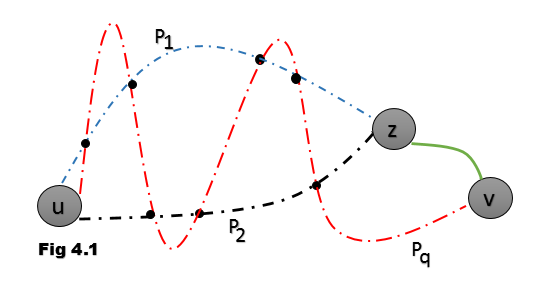
\includegraphics[scale = 0.327]{img/4fig1.png}
        \centering
    \end{figure}
    \noindent Sea G un grafo donde $\forall\; u,v\in V(G)\; d(u,v)=k>1$. Entonces en G existe un camino de longitud k entre 
    cualquier par de v\'ertices $u$,$v$. Sea z el \'ultimo v\'ertice anterior a v en el camino de de longitud k que va de
    $u$ a $v$ . Obtenemos $d(u,z)=d(u,v)-1=k-1$. Por hip\'otesis de inducci\'on existen dos caminos disjuntos en v\'ertices 
    $P_{1},P_{2}$ de $u$ a $v$. Dado que G-z es conexo pues G es biconexo ,entonces existe un camino $P_{q}$ que va de u a v
    y no contiene a z. Si $P_{q}$ no intersecta con $P_{1}$ o con $P_{2}$,tenemos los dos caminos disjuntos en v\'ertices
    de $u$ a $v$: $P_{q}$ y $P_{1}$ o $P_{2}$(uno de los 2 con el que no tiene intersecci\'on) + $<z,v>$. Digamos que $P_{q}$ intersecta 
    con $P_{1}$ y con $P_{2}$(posiblemente en m\'as de una ocasi\'on  a ambos), vamos a crear un camino que comienza en $v$ sigue por $P_{q}$ hasta la primera intersecci\'on con
    $P_{1}$ o $P_{2}$ y sigue por uno de estos dos hasta $u$, este camino no contiene a z. Ahora creamos  otro camino que vaya 
    desde $u$, por el camino que que no tomamos entre $P_{1}$ y $P_{2}$ en el camino previamente construido,  hasta z y con la arista $<z,v>$ llega 
    a $v$. Encontramos dos caminos disjuntos en v\'ertices que van de $u$ a $v$ $(fig4.1)$.\\\\
    Luego en G hay dos caminos disjuntos en v\'ertices de $u$ a $v$ $\forall u,v \in V(G)$\\\\
 
    \noindent \textbf{Lema 2:}\\
    G es biconexo $\Longleftrightarrow$ G no tiene puntos de articulaci\'on \\\\
    \noindent \textbf{Demostraci\'on:}\\
    $\Longrightarrow$\\
    Si G es biconexo entonces al quitar cualquier v\'ertice v de G, y las aristas incidentes al mismo,  
    G sigue siendo conexo por que lo no se divide en 2 o m\'as de componentes conexas. Por tanto G no
    tiene puntos de articulaci\'on.\\\\
    $\Longleftarrow$\\
    Si G no tiene puntos de articulaci\'on entonces no existe ning\'un  v\'ertice v que quite de G que lo separe en
    2 o m\'as componentes conexas. Entonces G-v sigue siendo conexo. Luego G es biconexo.\\\\
  
    
    \noindent \textbf{Lema 3:}\\
    Sea G un grafo con $V(G)\ge 3$ $\forall x,y\in V(G)$ existen dos caminos disjuntos en v\'ertices $\Longleftrightarrow$ G no tiene puntos de articulaci\'on\\\\
    \noindent \textbf{Demostraci\'on:}\\
    Por Lema 1  $\forall x,y\in V(G)$ con $|V(G)|\ge 3$ existen dos caminos disjuntos en v\'ertices $\Longleftrightarrow$ G es biconexo. 
    Por Lema 2 G es biconexo $\Longleftrightarrow$ G no tiene puntos de articulaci\'on.
    Entonces por transitividad $\forall x,y\in V(G)$ $|V(G)|\ge 3$ existen dos caminos disjuntos en v\'ertices 
    $\Longleftrightarrow$ G no tiene puntos de articulaci\'on\\\\
    
    \noindent \textbf{Caso  $|V(G)|\le 2$:}\\
    Si $|V(G)| = 2$, entonces el \'unico camino que puede existir entre los \'unicos dos v\'ertices u,v que tiene el grafo es la
    arista $<u,v>$, por lo que no cumple la condici\'on que nos pide en el problema. En este caso G nunca tiene puntos de articulaci\'on,
    pues cualquiera de los 2 v\'ertices que quitemos siempre quedar\'ia un grafo conexo de un solo v\'ertice, por lo que lo consideramos
    aparte en el algoritmo.\\
    Si $|V(G)| = 1$, entonces como G tiene un solo v\'ertice, no puede existir ning\'un camino en G hacia otro v\'ertice, por lo que tampoco safisface la condici\'on
    que nos pide problema.\\

    \subsection{\underline{Pseudoc\'odigo}}
    
    \begin{algorithm}[H] 
        Pseudoc\'odigo:
        \caption{Determinar si un grafo G cumple $\forall x,y\in V(G)$  existen dos caminos disjuntos en v\'ertices de x a y }
        \textbf{Solve($G$)\\}
        $answer=[\;]$ - lista para almacenar los puntos de articulaci\'on\\
        $childrens=[\;]$ - array para saber cuantos hijos tiene un v\'ertice que pertenece al \'arbol resultado de hacer DFS-Visit\\
        1-\hspace*{1em}\noindent \textbf{DFS-Visit-PA($G,u$)} \\ 
        2-\hspace*{2em}u $\leftarrow$ visited \\
        3-\hspace*{2em}$time=time+1$ \\
        4-\hspace*{2em}$d[u]=time$\\
        5-\hspace*{2em}$low[u]=d[u]$\\ 
        6-\hspace*{2em}\noindent \textbf{for each} v $\in$ $Adj[u]$\\
        7-\hspace*{3em}do \noindent \textbf{if} v not visited\\
        8-\hspace*{4em}$\pi[v] \leftarrow u$\\
        9-\hspace*{4em}$childrens[u] \leftarrow childrens[u]+1$\\
        10-\hspace*{4em}DFS-Visit-PA($G,v$)\\
        11-\hspace*{4em}$low[u]=min(low[u],low[v])$\\
        12-\hspace*{4em}\noindent \textbf{if} $low[v]\ge d[u]$\\
        13-\hspace*{5em}answer.add(u)\\
        14-\hspace*{3em}\noindent \textbf{else if} $\pi[u]\ne v$\\
        15-\hspace*{4em}$low[u]=min(low[u],d[v])$\\ 
        16-\hspace*{2em}return\\\\
        17-\hspace*{1em}\noindent \textbf{DFS-PA($G$)}\\
        18-\hspace*{2em}\noindent \textbf{for each} v $\in$ V(G)\\
        19-\hspace*{3em}do \noindent \textbf{if} not visited\\
        20-\hspace*{4em}DFS-Visit-PA(G,v)\\
        21-\hspace*{4em}\noindent \textbf{if} $childrens[v] \ge 2$ -en caso de que la ra\'iz v  sea art point \\
        22-\hspace*{5em}anwser.add(v)\\
        23-\hspace*{2em}return \\\\
        24-\hspace*{1em}\noindent \textbf{Solve($G$)}\\
        25-\hspace*{2em}\noindent \textbf{if} $|V(G)| < 3$ -caso aparte si G tiene menos de 3 v\'ertices\\ 
        26-\hspace*{3em}return False\\
        27-\hspace*{2em}DFS-PA($G$)\\
        28-\hspace*{2em}\noindent \textbf{if} $size(anwser) > 0$\\
        29-\hspace*{3em}return False\\
        30-\hspace*{2em}\noindent \textbf{else}\\
        31-\hspace*{3em}return True\\
                
    \end{algorithm}

    \subsection{\underline{Correctitud}} 
    Por lo expuesto con anterioridad en los lemas 1,2,3 y por la correctitud del algoritmo de detecci\'on de puntos de 
    articulaci\'on, podemos asegurar la correctitud de nuestro algoritmo para detectar si un grafo $G$ cumple la propiedad 
    de  que para cada par de v\'ertices existen dos caminos disjuntos en v\'ertices entre ellos, o sea con almacenar en una lista
    los puntos de articulaci\'on detectados por el algoritmo y verificar si la lista contiene alg\'un v\'ertice es suficiente.
    La modificaci\'on al algoritmo visto en conferencia es, en vez de imprimir el punto de articulaci\'on, simplemente lo
    almacenamos en una lista, lo que no afecta la correctitud del algoritmo.
    \\\\

    \subsection{\underline{Complejidad Temporal}} 
    La complejidad temporal de nuestro algoritmo es la complejidad temporal del algoritmo de detecci\'on de puntos 
    de articulaci\'on que es $O(|V|+|E|)$. La modificaci\'on que hicimos del c\'odigo de conferencia no afecta la 
    complejidad del algoritmo pues solo cambia imprimir el v\'ertice por agregar el v\'ertice a una lista, que es una
    operaci\'on $O(1)$. Luego, preguntar por el size de la lista para saber si se encontraron puntos de articulaci\'on 
    es O(1), por lo que la complejidad del algoritmo sigue siendo $O(|V|+|E|)$.
    \newline
    
    

\end{document} 